\setlength{\parindent}{0em}

\subsection{Supervised learning}

\textbf{Decision Trees} \label{subsec: decisiontree}
%Decision trees are a good manner to figure out, which parts of the data set have the most influence on the decision. Therefore labeled data is needed and we have given the strata. We used again \textbf{RapidMiner} for building trees based on different data sets. 
%
%\begin{figure}[!htbp]
%\centering
%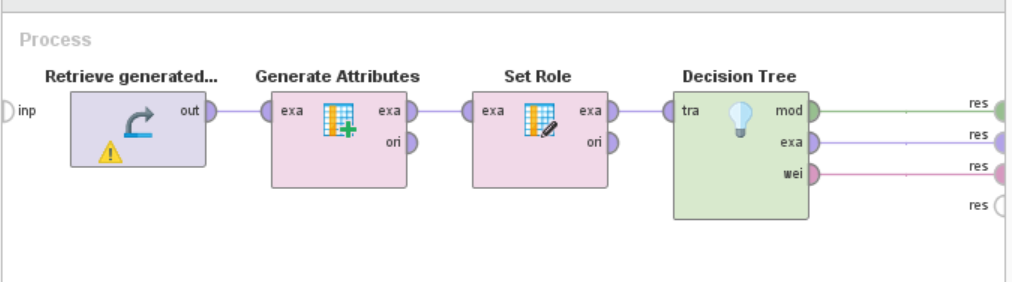
\includegraphics[width = 0.9\textwidth]{DecisionTreeRapidModel.PNG}
%\caption{Process for decision trees in RapidMiner}
%\label{fig: RapDec}
%\end{figure}
%
%RapidMiner does the following steps, to see in figure \ref{fig: RapDec}:
%\begin{description}
%	\item[Retrieve] includes the dataset
%	\item[Select Attributes] makes it possible to or have a look at grouped strata or normal strata
%	\item[Set Role] gives strata the label role, so that the decision tree has those as leafs
%	\item[Multiply] clones the data set 
%	\item[Decision Tree] creates the decision tree
%	\item[Apply Model] is used creates the labeled data set for the \textbf{Performance} step
%	\item[Performance] gives the performance result of the created model
%\end{description}
%
%Furthermore we choose information gain as splitting criterium (minimal gain 0.1) and a confidence of 0.25. Other configuration does not show different results.

In the first step we apply the process on the \textit{original data set} and the resulting tree is just the leaf `strata 2'. So we try it with different other data sets and the best result we get is for \textit{stratified person data} equally distributed and just 200 data entries in every strata.

\begin{figure}[H]
\centering
\begin{subfigure}{0.9\textwidth}
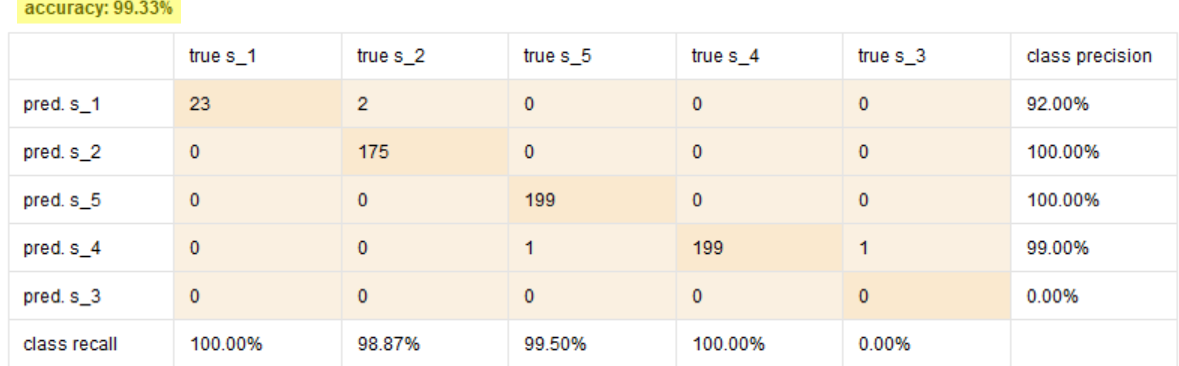
\includegraphics[width = \linewidth]{Dec200eqPrec.PNG}
\caption{200 in every strata}
\label{fig:decvec200}
\end{subfigure}
\begin{subfigure}{0.9\textwidth}
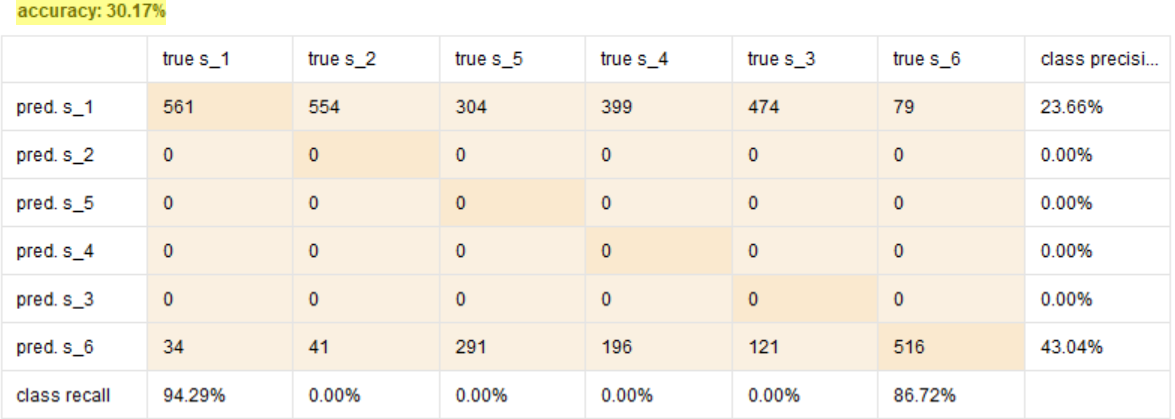
\includegraphics[width= \linewidth]{decvec585pre.PNG}
\caption{585 in every strata}
\label{fig:DecVec585}
\end{subfigure}
\caption{Performance for stratified person data}
\label{fig:DecVec}
\end{figure}

In \Cref{fig:DecVec} the best and worst outcome can be seen for 6 clusters. For all other configurations the outcome is similar, so just small data sets have an acceptable result and larger datasets have no sufficient results for our question.\\